%
\section{Introduction}\label{sec:introduction}
%
\subsection{Model description}
\label{subsec:model_description}
Like many other deep generative models, the variational auto encoders' (VAEs) aim is to learn the underlying input data distributions to generate new samples with features similar to the original ones. In order to achieve this goal, these algorithms are built basically in two steps: the first one - the \textit{encoding stage} - where the VAE compresses the input data in a lower-dimensional space (\textit{latent space}) and the second step where it tries to reconstruct the original input - \textit{decoding phase} - distribution starting from this incomplete information. \\Contrarily to the vanilla autoencoders, where a point wise encoding results in a less efficient and precise regeneration, the VAEs compress data in a continuous latent space. Indeed, each input is associated with a distribution within this space and the reconstruction step starts only after sampling from that distribution. In this way, the model is able to reconstruct similarly points close togheter in the latent space. This approach gives continuity and completeness to this space, making the regeneration step easier and more robust.

The variational autoencoder architecture could be thought of as the ensemble of two neural networks, one on top of the other, designed respectively with a contractive-path and an expansive one. The first of these provides a last layer/s with fewer neurons respect to the input layer, so to be able to compress the data in a lower-dimensional space. The second one, instead, starting from the latent representation, moves in the opposite direction and tries to reconstruct the compressed data in the higher-dimensional original space. Naturally, this separation is only speculative and joint optimization of all the network weights can be obtained minimizing an objective function.


The target \textit{function loss} suitable for the final goal is constituted by two pieces. The first term is related to the model reconstruction performances, while the second one regards the Kulback-Lieber divergence between the latent space shape and its target distribution, usually a multivariate standard gaussian. So the general form of the final loss results from a weighted sum of these two terms:

\begin{equation}\label{eq:1}
    Loss_{tot}=  Loss_{reco} + \beta D_{KL}
\end{equation}

where $\beta$ is a free parameter defining the relative weight of the divergence loss term in the total final score function and $D_{KL}$ is the Kulback-Lieber divergence, described in detail in Section~\ref{subsubsec:loss}. Under this loss definition, the model learns how to compress and successfully reconstruct the bulk of the variable distributions contained in the training samples. On the other hand, the model is prone to fail while reconstructing the more rare events. Due to this behavior, the latter kind of event is likely to end up in the right tail of the distribution loss (higher losses). This situation is even more evident when considering data samples characterized by different variable distributions with respect to the ones used for training, for example samples with non SM events which were not present in the SM-only background sample. \\Given these considerations, in this study a model trained to reproduce a cocktail of Monte Carlo SM processes is presented, with the aim of testing the background modeling capabilities. The signal sensitivity is tested including both background and signal events in the validation sample and expecting to find a region in the right tail of the loss distribution where maximize the purity of the signal.

\subsection{Dataset}
\label{subsec:dataset}

The Wh1Lbb analysis ntuples are used in this study. The same preselection of the original analysis~\cite{ATL-COM-PHYS-2018-1638} is applied both on the background processes and on the signal events and it is reported in Table~\ref{tab:preliminary_cuts}. In Figure~\ref{fig:feat_distr} the distributions of the most discriminating variables are shown for the total background (sum of all the processes) and some signal example. The definition and the data/MC agreement of each variable considered for the training are explained and described in detail in Section 6 of~\cite{ATL-COM-PHYS-2018-1638}. It is worth to remark that only the background events are used to train the model, while the signal events are only included in the evaluation step after the events selection.

\begin{table}[h]
\centering
\caption{Preselection cuts applied both on signal and background samples.}
\label{tab:preliminary_cuts}
\begin{tabular}{lc}
\hline
&Preselection \\
\hline
Exactly 1 signal lepton&True\\
met\ trigger fired&True\\
$2-3$ jets with $p_{T}>30 GeV$&True\\
$b$-tagged jet&[1-3]\\
met\ &$> 220$ GeV\\
mt\ &$> 50$ GeV\\
\hline
\end{tabular}
\end{table}

\begin{figure}
	\centering
  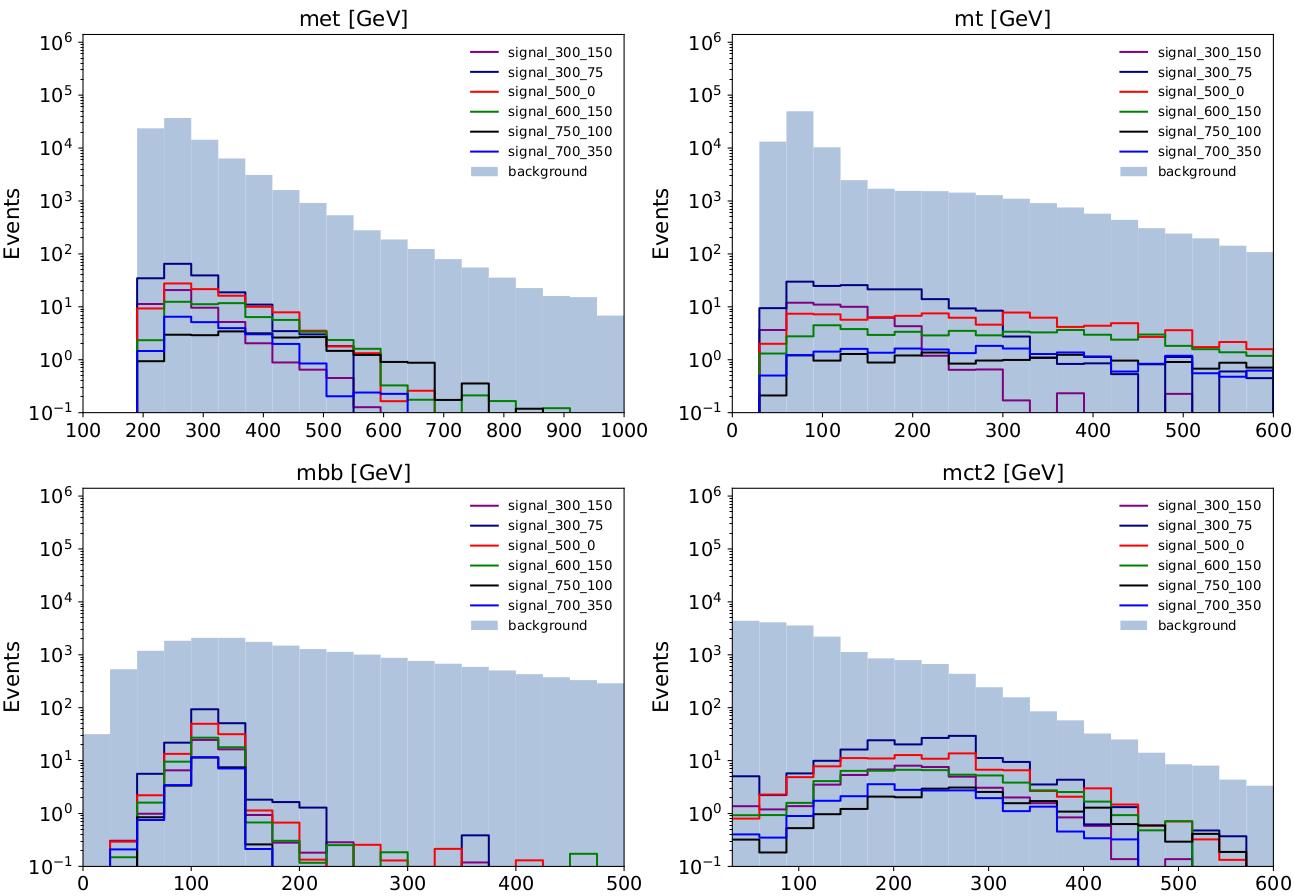
\includegraphics[width=0.85\textwidth]{figs/dataset/distr_1.png}
 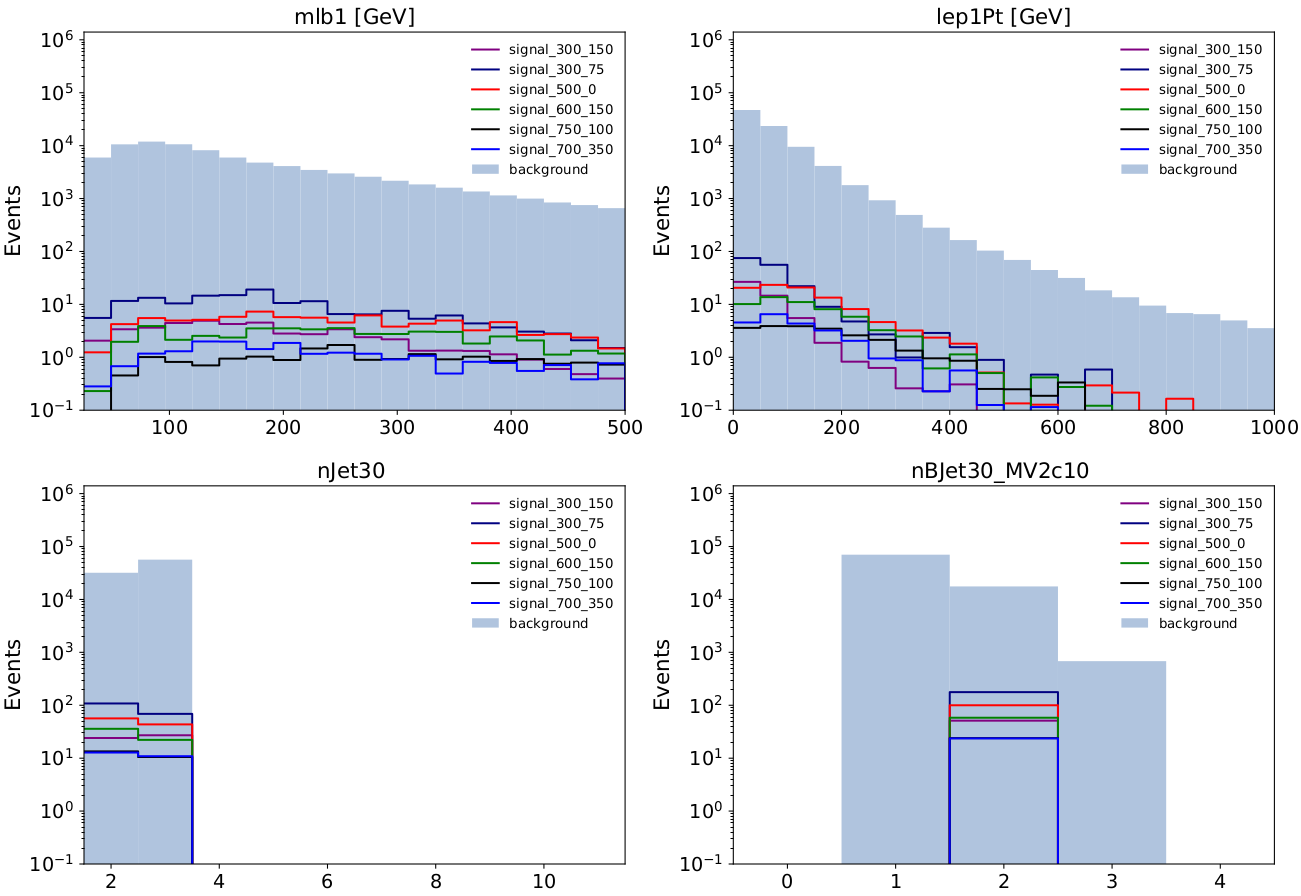
\includegraphics[width=0.85\textwidth]{figs/dataset/distr_2.png}
  \caption{Distributions of the input variables for the sum of all the background processes and some signal points, as example.}
  \label{fig:feat_distr}
\end{figure}

The model is trained in three different kinematics regions described in Table~\ref{tab:all_regions_cuts}. The aim is to test the sensitivity to the signal model in different topological spaces. The trade-off between a model-independent analysis and better signal sensitivity is one of the starting points investigated in this study. In the first case, any or only loose selection requirements would be applied to avoid cuts tailored on a specific signal hypothesis. Nevertheless, training on more selected background events could allow the model to focus more on the relevant background distinctive features finally leading to a better signal selection, albeit reducing the generality of the selection, and possibly reducing the selection sensitivity to similar models (as pMSSM, or different signal models).

\begin{table}[h]
\centering
\caption{Requirements for the three selected regions.}
\label{tab:all_regions_cuts}
\begin{tabular}{lccc}
\hline
&Preselection &mid. region &$2-3$b region\\
\hline
Exactly 1 signal lepton&True&True&True\\
met\ trigger fired&True&True&True\\
$2-3$ jets with $p_{T}>30 GeV$&True&True&True\\
$b$-tagged jet&[1-3]&[1-3]&[2-3]\\
met\ &$> 220$ GeV&$> 220$ GeV&$> 220$ GeV\\
mt\ &$> 50$ GeV&$> 50$ GeV&$> 50$ GeV\\
mbb\ &&$[100-140]$ GeV&$[100-140]$ GeV\\
mct\ &&$>100$ GeV&$>100$ GeV\\
\hline
\end{tabular}
\end{table}

\subsection{Training}
\label{subsec:training}

The model is trained in the three regions separately after a $60\%-40\%$ training-validation split. Due to the different selection depth, the total training-validation event number varies region by region. In order not to reduce this number drastically, a threshold of $10^{6}$ events for the training-validation sample is fixed as a lower limit and the \textit{$2$ - $3b$ region} is taken as the region with the smallest selected number of events.

\subsubsection{Loss function}
\label{subsubsec:loss}
The training loss function described above (eq. \ref{eq:1}) consists of two terms. The goal of the training is to find the best trade-off between good reconstruction performances and a regular latent space. A closer description of these two terms is given in the following.

The Kullback-Lieber divergence term regards the encoding phase outputs and forces all the predicted distributions to stay as close as possible to the prior choice. For the sake of simplicity, usually a multivariate gaussian is selected as target distribution. In this study, the Kulback-Lieber divergence has the following closed analytical form:

\begin{equation}\label{eq:2}
    D_{KL}=  \frac{1}{2k}  \sum_{i,j=1} \left( \sigma_{p}^{j}\sigma_{z}^{i,j} \right)^{2} +
\left( \frac{\mu_{p}^{j}\mu_{z}^{i,j}}{\sigma_{p}^{j}} \right)^{2} +
ln{\frac{\sigma_{p}^{j}}{\sigma_{z}^{i,j}}} -1 
\end{equation}

where,\textit{k} is the batch size selected for the training, \textit{i} runs over the samples and \textit{j} over the latent space dimensions. The parameters predicted from the model for each event are: $(1)$ $\mu_{z}$  and $\sigma_{z}$ that define the distribution shape in the latent space; $(2)$ $\mu_{p}$, and $\sigma_{p}$ that represents the prior shape parameters. It is important to observe that, following the work described in~\cite{vae:Cerri_2019}, also this latter couple of parameters are optimized during the training letting the model to select the optimal latent space target distribution.

The reconstruction loss term is instead represented by the average negative-log-likelihood of the inputs given the shape parameter values predicted by the model during the decoding phase:

\begin{align}\label{eq:3}
\begin{split}
    Loss_{reco}&=  -\frac{1}{k} \sum_{i,j=1} \ln \left[
    P\left(x| \alpha_{1}, \alpha_{2},...\alpha_{n}\right)
    \right]   \\
    &=  -\frac{1}{k} \sum_{i,j=1} \ln \left[
    f_{i,j}\left(x_{i,j}| \alpha_{1}^{i,j}, \alpha_{2}^{i,j},...\alpha_{n}^{i,j}\right)
    \right]   
\end{split}
\end{align}

In the equation, $\textit{j}$ runs over the input space dimensions, $\textit{$f_{i,j}$}$ is the functional form chosen to describe the pdf of the $\textit{i-th}$ input variable and $\alpha_{n}$ are the parameters of this function and represent also the final output of the network. Two different functional forms are selected to describe the distribution of the variables defining each physical events inside the training dataset. Specifically:

\begin{itemize}

\item the clipped log-normal function is used for all the continuous variables: \textit{met, mt, mbb, mct2, mlb1, lep1Pt}:

\begin{equation}\label{eq:4}
  P\left(x| \alpha_{1}, \alpha_{2},\alpha_{3} \right) =
    \begin{cases}
      \alpha_{3}\delta \left( x \right) \frac{1 - \alpha_{3}}{x\alpha_{2}+\sqrt{2\pi}} e^{-\frac{\left(\ln x -\alpha\right)^{2}}{2\alpha_{2}^{2}}}& for x \geq 10^{-4} \\
      0 & \leq 10^{-4}
 
    \end{cases}       
\end{equation}

\item A truncated discrete gaussian for for the discrete variables is: \textit{njet30, nBjet30\_MVc10}:

\begin{equation}\label{eq:5}
\Theta \left( x \right) \left[ erf \left(
          \frac{n + 0.5 - \alpha_{1}}{\alpha_{2}+\sqrt{2}}\right)
         - erf \left(\frac{n - 0.5 - \alpha_{1}}{\alpha_{2}+\sqrt{2}}\right)
\right]
\end{equation}

where the normalization factor N is set to:

\begin{equation}\label{eq:6}
N = \frac{1}{2}\left(
          \frac{-0.5 -\alpha_{1}}{\alpha_{2}+\sqrt{2}}\right)
\end{equation}

\end{itemize}

\subsubsection{Model architecture}
\label{subsubsec:model_architecture}

The network architecture is briefly described in the \ref{subsec:model_description}. It consists mainly of a contractive path followed by an expansive one. So, the feed-forward step goes first through a stack of fully-connected layers that progressively builds a representation of the inputs in the latent space and, then, towards a second fully-connected set of layers whose goal is to output the parameters shape (eq: \ref{eq:4}, \ref{eq:5}): the latter are used to describe the variables probability distributions for each event and represent the final output of the variational autoencoder.

The configuration of the network here trained is strongly inspired by the work \cite{vae:Cerri_2019}.

%% non capisco puoi spiegare meglio questa parte?

%% Rob: ho rispiegato un po', spero meglio

Nevertheless, the model configuration is also affected by the choice of a set of hyperparameters: that is, all the parameters fixed a priori, whose value is not learned automatically during the training. The hyperparameters are opposed to the network weights, linking the neurons in the model architecture for which an optimization occurs through the backpropagation of the loss. The weights update happens batch by batch during the traininig, following the gradient descents related to the loss minimization. The training success also depends on the hyperparameters that,  in some way, fix the boundary condition of the learning procedure. Usually, their choice proceeds by trial and error, but some hints to address the initial guesses come from the problem context. For example, increasing the number of hidden layers goes along the complexity of the model to be related to the dataset size. A more detailed list of hyperparameter examples is reported here:

\begin{itemize}
\item learning rate;
\item number of neurons per layer;
\item latent space dimension;
\item batch size;
\item beta weight in the total loss sum;
\item kind of activation layer;
\item penalization weights on one/more variable loss.
\end{itemize}

The list is quite long, and it is helpful to figure out how to handle the fine-tuning process in an effective way. For that reason, the \textit{tune} python library has been exploited and modified accordingly to work for this study. One of the strengths of this library is the possibility to run a hyperparameters optimization at any scale. Deploying on a cluster of many GPUs, as in this case, allows for an extensive search among all the possible parameters configuration, reducing the time and the human effort. A training summary is stored during the training and all the model performances can be compared. A final rank based on the evaluation metric helps to focus on the more promising architectures and, finally, to select the best one.
